%  article.tex (Version 3.3, released 19 January 2008)
%  Article to demonstrate format for SPIE Proceedings
%  Special instructions are included in this file after the
%  symbol %>>>>
%  Numerous commands are commented out, but included to show how
%  to effect various options, e.g., to print page numbers, etc.
%  This LaTeX source file is composed for LaTeX2e.

%  The following commands have been added in the SPIE class 
%  file (spie.cls) and will not be understood in other classes:
%  \supit{}, \authorinfo{}, \skiplinehalf, \keywords{}
%  The bibliography style file is called spiebib.bst, 
%  which replaces the standard style unstr.bst.  

\documentclass[letter]{spie}  %>>> use for US letter paper
%%\documentclass[a4paper]{spie}  %>>> use this instead for A4 paper
%%\documentclass[nocompress]{spie}  %>>> to avoid compression of citations
%% \addtolength{\voffset}{9mm}   %>>> moves text field down
%% \renewcommand{\baselinestretch}{1.65}   %>>> 1.65 for double spacing, 1.25 for 1.5 spacing 

%% Latex documents that need direct input

%  The following command loads a graphics package to include images 
%  in the document. It may be necessary to specify a DVI driver option,
%  e.g., [dvips], but that may be inappropriate for some LaTeX 
%  installations.
\usepackage{epsf,graphicx}
\usepackage{epstopdf}
\usepackage{subfig}

% Clever cross referencing. Using cleverref, instead of writting 
% figure~\ref{...} or equation~\ref{...}, only \cref{...} is required.
% The package interprates the references and introduces the figure, fig.,
% equation, eq., etc keywords. \Cref forces first letter capital. 
\usepackage{cleveref}

% In order to include files without having a clear page using \include*, 
% the newclude package is required
\usepackage{newclude}

% Required for acronyms
\usepackage{acro}

% For multirow environment
\usepackage{multirow}

% To use subscript environment
\usepackage{fixltx2e}

% Packages and defintion for tick and cross
\usepackage{pifont}
\newcommand{\cmark}{\large \color{green!60!black!80}\ding{51}}
\newcommand{\xmark}{\large \color{red!60!black!80}\ding{55}}
\newcommand{\cmarksmall}{\color{green!60!black!80}\ding{51}}
\newcommand{\xmarksmall}{\color{red!60!black!80}\ding{55}}

%% In order to draw some graphs
\usepackage{tikz,xifthen}
\usepackage{tikz-qtree}
\usetikzlibrary{decorations.pathmorphing} % noisy shapes
\usetikzlibrary{fit}                                            % fitting shapes to coordinates
\usetikzlibrary{backgrounds}                                    % drawing the background after the foreground
\usetikzlibrary{shapes,arrows,shadows}
\usetikzlibrary{calc,decorations.pathreplacing,decorations.markings,positioning}
\usetikzlibrary{snakes,decorations.text,shapes,patterns}        % contains the latex packages

\title{A boosting approach for prostate cancer detection using multi-parametric MRI} 

%>>>> The author is responsible for formatting the 
%  author list and their institutions.  Use  \skiplinehalf 
%  to separate author list from addresses and between each address.
%  The correspondence between each author and his/her address
%  can be indicated with a superscript in italics, 
%  which is easily obtained with \supit{}.

% \author{Anna A. Author1\supit{a} and Barry B. Author2\supit{b}
% \skiplinehalf
% \supit{a}Affiliation1, Address, City, Country; \\
% \supit{b}Affiliation2, Address, City, Country
% }

\author{Guillaume~Lema\^{i}tre\supit{a,c} and
                Joan~Massich\supit{a} and
                Robert~Mart\'{i}\supit{c} and
                Jordi~Freixenet\supit{c} and
                Joan~C.~Vilanova\supit{d} and
                Paul~M.~Walker\supit{b} and
                D\'esir\'e~D.~Sidib\'e\supit{a} and
                Fabrice~M\'{eriaudeau}\supit{a}
  \skiplinehalf
  \supit{a}{\scriptsize LE2I-UMR CNRS 6306, Universit\'{e} de Bourgogne, 12 rue de la Fonderie, 71200 Le Creusot, France;} \\
  \supit{b}{\scriptsize LE2I-UMR CNRS 6306, Universit\'{e} de Bourgogne, Avenue Alain Savary, 21000 Dijon, France;} \\
  \supit{c}{\scriptsize ViCOROB, Universitat de Girona, Campus Montilivi, Edifici P4, 17071 Girona, Spain;}\\
  \supit{d}{\scriptsize Department of Magnetic Resonance, Clinica Girona, Lorenzana 36, 17002 Girona, Spain} \\
}

%>>>> Further information about the authors, other than their 
%  institution and addresses, should be included as a footnote, 
%  which is facilitated by the \authorinfo{} command.

\authorinfo{Further author information: (Send correspondence to G.L.)\\G.L.: E-mail: guillaume.lemaitre@udg.edu}
%%>>>> when using amstex, you need to use @@ instead of @

%%% Local Variables: 
%%% mode: latex
%%% TeX-master: "../master.tex"
%%% End:              % contains the Title and Autor info
%%%%%%%%%%%%%%%%%%%%%%%%%%%%%%%%%%%%%%%%%%%%%%%%%%%%%%%%%%%%% 
%>>>> uncomment following for page numbers
% \pagestyle{plain}    
%>>>> uncomment following to start page numbering at 301 
%\setcounter{page}{301} 
      % contains package and variables init.
%% Acronym definition example using glossaries package
%% \usepackage{acro} is required
%% 
%% For a powerful usage of the acro package look at http://tex.stackexchange.com/questions/135975/how-to-define-an-acronym-by-using-other-acronym-and-print-the-abbreviations-toge

\DeclareAcronym{myac}{
  short = mA,
  long  = my Acronym
}
      % contains the acronims 

%% Select inputing only one part of the document
%\includeonly{content/intro/intro}   % the file wihtout .tex
%\includeonly{content/other/other_content}
 
\begin{document} 
\maketitle 

\begin{abstract}
Prostate cancer has been reported as the second most frequently diagnosed men cancers in the world. In the last decades, new imaging techniques based on MRI have been developed in order to improve the diagnosis task of radiologists. In practise, diagnosis can be affected by multiple factors reducing the chance to detect potential lesions. Computer-aided detection and computer-aided diagnosis have been designed to answer to these needs and provide help to radiologists in their daily duties. In this study, we proposed an automatic method to detect prostate cancer from a per voxel manner using 3T multi-parametric MRI and a gradient boosting classifier. The best performances are obtained using all multi-parametric information as well as zonal information. The sensitivity and specificity obtained are 86.9\% and 84.6\%, respectively.
\end{abstract}

\keywords{Gradient boosting, multi-parametric MRI, prostate cancer, computer-aided diagnosis}

%% Incldue the content without .tex extension
\section{INTRODUCTION}\label{sec:introduction}

On a worldwide scale, \ac{cap} has been reported as the second most frequently diagnosed men cancers accounting for 13.6\,\%~\cite{Ferlay2010}. Statistically, the estimated number of new diagnosed cases was 899,000 with no less than 258,100 estimated deaths~\cite{Ferlay2010}. In United States, aside from skin cancer, \ac{cap} was declared to be the most commonly diagnosed cancer among men, implying that around one in seven men will be diagnosed with \ac{cap} during their lifetime~\cite{Siegel2014}.

Since its introduction in mid-1980s, \ac{psa} is widely used for \ac{cap} screening~\cite{Etzioni2002} and has shown to improve early detection of \ac{cap}~\cite{Chou2011}. However, several trials conducted in Europe and United States conclude that \ac{psa} screening suffers from low specificity~\cite{Andriole2009,Hugosson2010,Schroeder2012}. Thus, current research focus on developing new screening methods to improve \ac{cap} detection. In this perspective, \Ac{mri} techniques have recently shown promising results for \ac{cap} detection. Furthermore, three different modalities are currently investigated: (i) \ac{t2w} \ac{mri}, (ii) \ac{dce} \ac{mri} and (iii) \ac{dw} \ac{mri}.

Several researches have been carried out in order to investigate the contributions of machine learning classifiers for \ac{cap} detection using the three aforementioned 3T multi-parametric \ac{mri} such as \ac{svm}~\cite{Litjens2011,Litjens2012a,Litjens2014,Liu2013,Peng2013}, probabilistic boosting tree~\cite{Viswanath2011} or probabilistic neural network~\cite{Viswanath2011}. However, these studies use different datasets and evaluation statistics to report their results leading to an impossibility to give rise to a fair comparison.

In this research, we investigate the performance of gradient boosting for \ac{cap} detection using 3T multi-parametric \ac{mri}. Two different features extraction strategies have been chosen in order to feed the classifier: (i) voxel-based and (ii) 3D texton-based. An evaluation of both strategies as well as the contribution of each modality is provided. Furthermore, the dataset used for this experimentation is part of our future benchmarking platform I2CVB available at {\tt http://visor.udg.edu/i2cvb/} and are available for future comparisons.

%%% Local Variables: 
%%% mode: latex
%%% TeX-master: "../../master.tex"
%%% End:    % the file wihtout .tex
\section{MATERIAL AND METHODS}\label{sec:methodology}


\subsection{Data}\label{subsec:data}

Here, right a paragraph on how the data were acquired and which features were extracted

\subsection{Classification framework}

\subsubsection{Feature extraction strategies}

\begin{itemize}
\item voxel-based
\item 3d-texton-based
\end{itemize}

\subsubsection{Gradient boosting}

\subsection{Validation model}

k-cross validation

%%% Local Variables: 
%%% mode: latex
%%% TeX-master: "../../master.tex"
%%% End: 
\section{RESULTS AND DISCUSSION}\label{sec:results}

%% Figure 1
\begin{figure}[t]
%%Figure1a
\subfloat[Voxel-based features]{\label{fig:voxres}
\hspace{0.8cm}
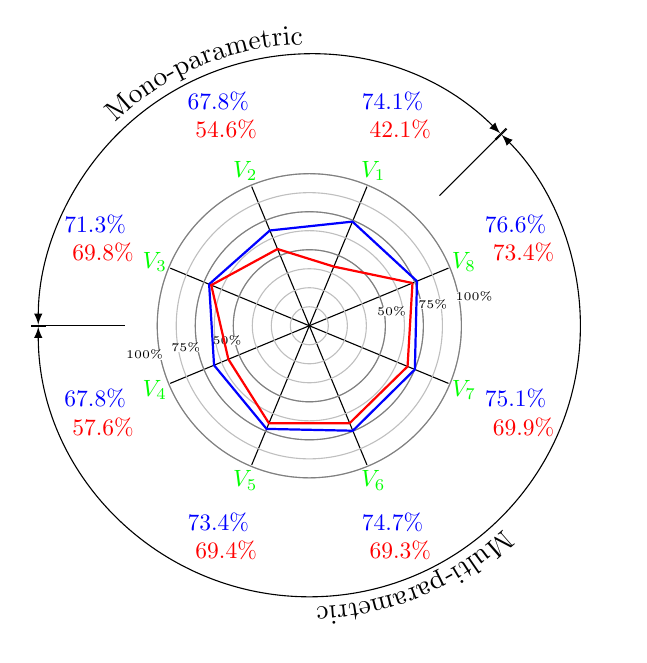
\begin{tikzpicture} [scale=.85,every node/.style={scale=0.85}]  %[scale=.68]

\def\labels{
{\color{green}$V_{1}$}, 
{\color{green}$V_{2}$}, 
{\color{green}$V_{3}$},  
{\color{green}$V_{4}$},
{\color{green}$V_{5}$},
{\color{green}$V_{6}$},
{\color{green}$V_{7}$},
{\color{green}$V_{8}$}
 }

\def\reward{74.1,67.8,71.3,67.8,73.4,74.7,75.1,76.6}
\def\spec{42.1,54.6,69.8,57.6,69.4,69.3,69.9,73.4}
\def\cZoom{2.5} 
\def\percentageLabelAngle{10}
\def\nbeams{8}
\pgfmathsetmacro\beamAngle{(360/\nbeams)}
\pgfmathsetmacro\halfAngle{(180/\nbeams)}

\pgfmathsetmacro\globalRotation{\halfAngle}

\foreach \n  [count=\ni] in \labels
{
\pgfmathsetmacro\cAngle{{(\ni*(360/\nbeams))+\globalRotation}}
\draw(\cAngle:{\cZoom*1.00})  node[fill=white] {\n};
\draw [thin] (0,0) -- (\cAngle:{\cZoom*0.9}) ;

}

%% draw the % rings 
\foreach \x in {12.5,25, ...,100} 
\draw [thin,color=gray!50] (0,0) circle [radius={\cZoom*\x/110}];

\foreach \x in {50,75,100}
{ 
     \draw [thin,color=black!50] (0,0) circle [radius={\cZoom/110*\x}];
     \foreach \a in {0, 180} \draw ({\percentageLabelAngle+\a}:{\cZoom*0.01*\x}) node  [inner sep=0pt,outer sep=0pt,fill=white,font=\fontsize{3}{3.5}\selectfont]{$\x\%$};
}

%% draw the path of the percentages
\def\aux{{\reward}}
\pgfmathsetmacro\origin{\aux[\nbeams-1]} 
\draw [blue, thick] (\globalRotation:{\cZoom*\origin/110}) \foreach \n  [count=\ni] in \reward { -- ({(\ni*(360/\nbeams))+\globalRotation}:{\cZoom*\n/110}) } ;

\def\auxx{{\spec}}
\pgfmathsetmacro\origin{\auxx[\nbeams-1]} 
\draw [red, thick] (\globalRotation:{\cZoom*\origin/110}) \foreach \n  [count=\ni] in \spec { -- ({(\ni*(360/\nbeams))+\globalRotation}:{\cZoom*\n/110}) };


\foreach \n [count=\ni] in \reward 
{
  \pgfmathsetmacro\cAngle{{(\ni*(360/\nbeams))+\globalRotation}}
  \pgfmathsetmacro\nreward{\aux[\ni-1]}
  \pgfmathsetmacro\nspec{\auxx[\ni-1]}
  \draw (\cAngle:{\cZoom*1.36}) node[align=center] {{\color{blue}\nreward $\%$ } \\{ \color{red}\nspec $\%$}};
};

%%%% draw the domain of each class 
\def\puta{3/0/{Mono-parametric},
  5/3/{Multi-parametric}}
\foreach \numElm/\contadorQueNoSeCalcular/\name [count=\ni] in \puta
 {

   \pgfmathsetmacro\initialAngle{(\contadorQueNoSeCalcular*\beamAngle)+\halfAngle+\globalRotation}
   \pgfmathsetmacro\finalAngle  {((\numElm+\contadorQueNoSeCalcular)*\beamAngle)+\halfAngle+\globalRotation}
   \pgfmathsetmacro\l  {\cZoom*1.5+.3pt}
   \draw (\initialAngle:{\cZoom*1.6}) -- (\initialAngle:{\cZoom*1.1});
   \draw [ |<->|,>=latex] (\initialAngle:\l) arc (\initialAngle:\finalAngle:\l) ;     
   \pgfmathsetmacro\r  {\cZoom*1.5+.45pt}
   {\draw [decoration={text along path,  text={\name},text align={center}},decorate] (\finalAngle:\r) arc (\finalAngle:\initialAngle:\r);} 
    
  }  
\end{tikzpicture} 
}\hfill
%%Figure1b
\subfloat[3D texton-based features]{\label{fig;texres}
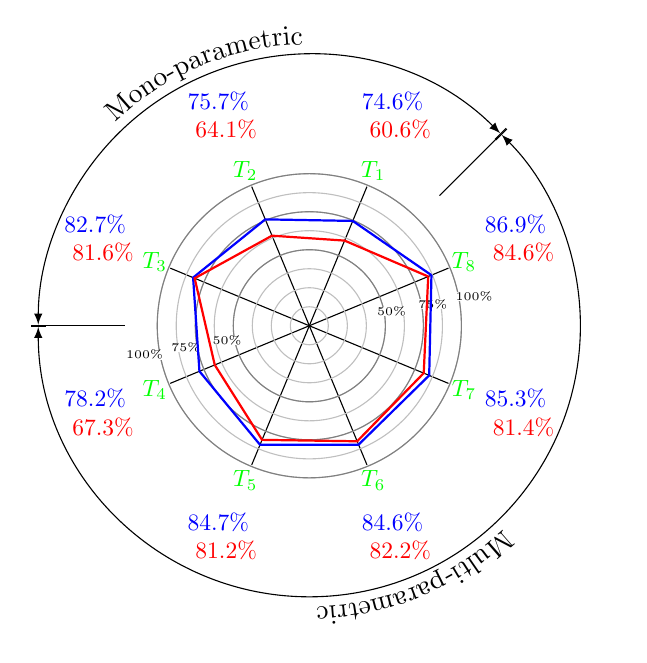
\begin{tikzpicture} [scale=.85,every node/.style={scale=0.85}]  %[scale=.68]

\def\labels{
{\color{green}$T_{1}$}, 
{\color{green}$T_{2}$}, 
{\color{green}$T_{3}$},  
{\color{green}$T_{4}$},
{\color{green}$T_{5}$},
{\color{green}$T_{6}$},
{\color{green}$T_{7}$},
{\color{green}$T_{8}$}
 }

\def\reward{74.6,75.7,82.7,78.2,84.7,84.6,85.3,86.9}
\def\spec{60.6,64.1,81.6,67.3,81.2,82.2,81.4,84.6}
\def\cZoom{2.5} 
\def\percentageLabelAngle{10}
\def\nbeams{8}
\pgfmathsetmacro\beamAngle{(360/\nbeams)}
\pgfmathsetmacro\halfAngle{(180/\nbeams)}

\pgfmathsetmacro\globalRotation{\halfAngle}

\foreach \n  [count=\ni] in \labels
{
\pgfmathsetmacro\cAngle{{(\ni*(360/\nbeams))+\globalRotation}}
\draw(\cAngle:{\cZoom*1.00})  node[fill=white] {\n};
\draw [thin] (0,0) -- (\cAngle:{\cZoom*0.9}) ;

}

% draw the % rings 
\foreach \x in {12.5,25, ...,100} 
\draw [thin,color=gray!50] (0,0) circle [radius={\cZoom*\x/110}];

\foreach \x in {50,75,100}
{ 
     \draw [thin,color=black!50] (0,0) circle [radius={\cZoom/110*\x}];
     \foreach \a in {0, 180} \draw ({\percentageLabelAngle+\a}:{\cZoom*0.01*\x}) node  [inner sep=0pt,outer sep=0pt,fill=white,font=\fontsize{3}{3.5}\selectfont]{$\x\%$};
}


% draw the path of the percentages
\def\aux{{\reward}}
\pgfmathsetmacro\origin{\aux[\nbeams-1]} 
\draw [blue, thick] (\globalRotation:{\cZoom*\origin/110}) \foreach \n  [count=\ni] in \reward { -- ({(\ni*(360/\nbeams))+\globalRotation}:{\cZoom*\n/110}) } ;


\def\auxx{{\spec}}
\pgfmathsetmacro\origin{\auxx[\nbeams-1]} 
\draw [red, thick] (\globalRotation:{\cZoom*\origin/110}) \foreach \n  [count=\ni] in \spec { -- ({(\ni*(360/\nbeams))+\globalRotation}:{\cZoom*\n/110}) };

% label all the percentags
\foreach \n [count=\ni] in \reward 
{
  \pgfmathsetmacro\cAngle{{(\ni*(360/\nbeams))+\globalRotation}}
  \pgfmathsetmacro\nreward{\aux[\ni-1]}
  \pgfmathsetmacro\nspec{\auxx[\ni-1]}
  \draw (\cAngle:{\cZoom*1.36}) node[align=center] {{\color{blue}\nreward $\%$ } \\{ \color{red}\nspec $\%$}};
};

%%% draw the domain of each class 
\def\puta{3/0/{Mono-parametric},
  5/3/{Multi-parametric}}
\foreach \numElm/\contadorQueNoSeCalcular/\name [count=\ni] in \puta
 {
   \pgfmathsetmacro\initialAngle{(\contadorQueNoSeCalcular*\beamAngle)+\halfAngle+\globalRotation}
   \pgfmathsetmacro\finalAngle  {((\numElm+\contadorQueNoSeCalcular)*\beamAngle)+\halfAngle+\globalRotation}
   \pgfmathsetmacro\l  {\cZoom*1.5+.3pt}
   \draw (\initialAngle:{\cZoom*1.6}) -- (\initialAngle:{\cZoom*1.1});
   \draw [ |<->|,>=latex] (\initialAngle:\l) arc (\initialAngle:\finalAngle:\l) ;     
   \pgfmathsetmacro\r  {\cZoom*1.5+.45pt}
   {\draw [decoration={text along path,  text={\name},text align={center}},decorate] (\finalAngle:\r) arc (\finalAngle:\initialAngle:\r);}     
  }  
\end{tikzpicture}
}
\caption{Comparison between the combination of features introduced in Table~\ref{tab:conc} in terms of sensitivity and specificity are illustrated in {\color{blue}blue} and {\color{red}red}, respectively.} 
\label{fig:result}
\end{figure}

%%% Local Variables: 
%%% mode: latex
%%% TeX-master: "../../master.tex"
%%% End: 

The classification results obtained are depicted in Fig.\,\ref{fig:result}. The best classification performances are achieved the 3D texton-based extraction strategy and a combination of the three different modalities and the zonal information. The sensitivity and specificity obtained are 86.9\% and 84.6\%, respectively.

Analyzing the classification outcomes of each single modality, the \ac{adc} map is the most discriminative feature with superior performances than the combination of \ac{t2w} \ac{mri} and \ac{dce} \ac{mri} together. However, the two latter mentioned modalities provide relevant information since that the combination of the three of them enhances the reported sensitivity and specificity. 

Integrating information about the prostate zones (i.e., \ac{pz} and \ac{cg}) boosts the classification performances. More precisely, this feature allows to improve greatly the specificity and slightly the sensitivity. 

In overall, the 3D texton-based strategy leads to better classification results compared with the voxel-based strategy for all the mono and multi parametric combinations experimented. Thus, integrating spatial information about the neighborhood of a given voxel should lead to drastic improvements.

%%% Local Variables: 
%%% mode: latex
%%% TeX-master: "../../master.tex"
%%% End: 
%\section{DISCUSSION}\label{sec:discussion}


%%% Local Variables: 
%%% mode: latex
%%% TeX-master: "../../master.tex"
%%% End: 
\section{CONCLUSION}\label{sec:conclusion}

In this study, an exhaustive analysis of classification of 3T multi-parametric \ac{mri} data using a gradient boosting classifier has been carried out. The best classification performances are obtained by extracting the features using a 3D texton-based strategy and using the information from all the modalities as well as the zonal information. A maximum sensitivity and specificity of 86.9\% and 84.6\% respectively, are reached.

Two avenues for research can be explored. First, the registration of the multi-parametric data has been discarded and could be performed ahead of the classification to study the possible improvements implied. Then, other features than intensities could be extracted and results could be compared with the experiments here described since that our dataset in public.

%%% Local Variables: 
%%% mode: latex
%%% TeX-master: "../../master.tex"
%%% End: 

\acknowledgments     %>>>> equivalent to \section*{ACKNOWLEDGMENTS}       

Guillaume Lema\^itre was supported by the Generalitat de Catalunya (grant nb. FI-DGR2012) and partly by the Mediterranean Office for Youth (grant nb. 2011/018/06). We would like also to thank the Clinica Girona (Catalunya,
Espanya) and the Centre Hospitalier of Dijon (France) for providing the MRI images used in this research.


\section*{BIOGRAPHY}

Guillaume Lemaitre received an Erasmus Mundus MSc in Vision and Robotic (ViBOT) from the Heriot-Watt University, Universit\'e de Bourgone and Universitat de Girona as well as a MSc in Business Innovation and Technology Management (BITM) from the Universitat de Girona. He is currently carrying out a joint PhD at the Universit\'e de Bourgogne and Universitat de Girona focusing on the development of computer-aided diagnosis for prostate cancer. 

%%% Local Variables: 
%%% mode: latex
%%% TeX-master: "../../master"
%%% End: 


%%%%%%%%%%%%%%%%%%%%%%%%%%%%%%%%%%%%%%%%%%%%%%%%%%%%%%%%%%%%%
%%%%% References %%%%%

\bibliography{./content/literature_review}   %>>>> bibliography data in report.bib
\bibliographystyle{spiebib}   %>>>> makes bibtex use spiebib.bst

\end{document} 
